%% (Master) Thesis template
% Template version used: v1.4
%
% Largely adapted from Adrian Nievergelt's template for the ADPS
% (lecture notes) project.


%% We use the memoir class because it offers a many easy to use features.
\documentclass[11pt,a4paper,titlepage,oneside]{memoir}

%% Packages
%% ========

%% LaTeX Font encoding -- DO NOT CHANGE
\usepackage[OT1]{fontenc}

%% Babel provides support for languages.  'english' uses British
%% English hyphenation and text snippets like "Figure" and
%% "Theorem". Use the option 'ngerman' if your document is in German.
%% Use 'american' for American English.  Note that if you change this,
%% the next LaTeX run may show spurious errors.  Simply run it again.
%% If they persist, remove the .aux file and try again.
\usepackage[english]{babel}

%% Input encoding 'utf8'. In some cases you might need 'utf8x' for
%% extra symbols. Not all editors, especially on Windows, are UTF-8
%% capable, so you may want to use 'latin1' instead.
\usepackage[utf8]{inputenc}

%% This changes default fonts for both text and math mode to use Herman Zapfs
%% excellent Palatino font.  Do not change this.
\usepackage[sc]{mathpazo}

%% The AMS-LaTeX extensions for mathematical typesetting.  Do not
%% remove.
\usepackage{amsmath,amssymb,amsfonts,mathrsfs}

%% NTheorem is a reimplementation of the AMS Theorem package. This
%% will allow us to typeset theorems like examples, proofs and
%% similar.  Do not remove.
%% NOTE: Must be loaded AFTER amsmath, or the \qed placement will
%% break
\usepackage[amsmath,thmmarks]{ntheorem}

%% LaTeX' own graphics handling
\usepackage{graphicx}

%% We unfortunately need this for the Rules chapter.  Remove it
%% afterwards; or at least NEVER use its underlining features.
\usepackage{soul}

%% This allows you to add .pdf files. It is used to add the
%% declaration of originality.
\usepackage{pdfpages}

%% Some more packages that you may want to use.  Have a look at the
%% file, and consult the package docs for each.
%% See the TeXed file for more explanations

%% [OPT] Multi-rowed cells in tabulars
%\usepackage{multirow}

%% [REC] Intelligent cross reference package. This allows for nice
%% combined references that include the reference and a hint to where
%% to look for it.
\usepackage{varioref}

%% [OPT] Easily changeable quotes with \enquote{Text}
%\usepackage[german=swiss]{csquotes}

%% [REC] Format dates and time depending on locale
\usepackage{datetime}

%% [OPT] Provides a \cancel{} command to stroke through mathematics.
%\usepackage{cancel}

%% [NEED] This allows for additional typesetting tools in mathmode.
%% See its excellent documentation.
\usepackage{mathtools}

%% [ADV] Conditional commands
%\usepackage{ifthen}

%% [OPT] Manual large braces or other delimiters.
%\usepackage{bigdelim, bigstrut}

%% [REC] Alternate vector arrows. Use the command \vv{} to get scaled
%% vector arrows.
\usepackage[h]{esvect}

%% [NEED] Some extensions to tabulars and array environments.
\usepackage{array}

%% [OPT] Postscript support via pstricks graphics package. Very
%% diverse applications.
%\usepackage{pstricks,pst-all}

%% [?] This seems to allow us to define some additional counters.
%\usepackage{etex}

%% [ADV] XY-Pic to typeset some matrix-style graphics
%\usepackage[all]{xy}

%% [OPT] This is needed to generate an index at the end of the
%% document.
%\usepackage{makeidx}

%% [OPT] Fancy package for source code listings.  The template text
%% needs it for some LaTeX snippets; remove/adapt the \lstset when you
%% remove the template content.
\usepackage{listings}
\lstset{language=TeX,basicstyle={\normalfont\ttfamily}}

%% [REC] Fancy character protrusion.  Must be loaded after all fonts.
\usepackage[activate]{pdfcprot}

%% [REC] Nicer tables.  Read the excellent documentation.
\usepackage{booktabs}


%% Our layout configuration.  DO NOT CHANGE.
%% Memoir layout setup

%% NOTE: You are strongly advised not to change any of them unless you
%% know what you are doing.  These settings strongly interact in the
%% final look of the document.

% Dependencies
\usepackage{utils/ETHlogo}

% Turn extra space before chapter headings off.
\setlength{\beforechapskip}{0pt}

\nonzeroparskip
\parindent=0pt
\defaultlists

% Chapter style redefinition
\makeatletter

\if@twoside
  \pagestyle{Ruled}
  \copypagestyle{chapter}{Ruled}
\else
  \pagestyle{ruled}
  \copypagestyle{chapter}{ruled}
\fi
\makeoddhead{chapter}{}{}{}
\makeevenhead{chapter}{}{}{}
\makeheadrule{chapter}{\textwidth}{0pt}
\copypagestyle{abstract}{empty}

\makechapterstyle{bianchimod}{%
  \chapterstyle{default}
  \renewcommand*{\chapnamefont}{\normalfont\Large\sffamily}
  \renewcommand*{\chapnumfont}{\normalfont\Large\sffamily}
  \renewcommand*{\printchaptername}{%
    \chapnamefont\centering\@chapapp}
  \renewcommand*{\printchapternum}{\chapnumfont {\thechapter}}
  \renewcommand*{\chaptitlefont}{\normalfont\huge\sffamily}
  \renewcommand*{\printchaptertitle}[1]{%
    \hrule\vskip\onelineskip \centering \chaptitlefont\textbf{\vphantom{gyM}##1}\par}
  \renewcommand*{\afterchaptertitle}{\vskip\onelineskip \hrule\vskip
    \afterchapskip}
  \renewcommand*{\printchapternonum}{%
    \vphantom{\chapnumfont {9}}\afterchapternum}}

% Use the newly defined style
\chapterstyle{bianchimod}

\setsecheadstyle{\Large\bfseries\sffamily}
\setsubsecheadstyle{\large\bfseries\sffamily}
\setsubsubsecheadstyle{\bfseries\sffamily}
\setparaheadstyle{\normalsize\bfseries\sffamily}
\setsubparaheadstyle{\normalsize\itshape\sffamily}
\setsubparaindent{0pt}

% Set captions to a more separated style for clearness
\captionnamefont{\sffamily\bfseries\footnotesize}
\captiontitlefont{\sffamily\footnotesize}
\setlength{\intextsep}{16pt}
\setlength{\belowcaptionskip}{1pt}

% Set section and TOC numbering depth to subsection
\setsecnumdepth{subsection}
\settocdepth{subsection}

%% Titlepage adjustments
\pretitle{\vspace{0pt plus 0.7fill}\begin{center}\HUGE\sffamily\bfseries}
\posttitle{\end{center}\par}
\preauthor{\par\begin{center}\let\and\\\Large\sffamily}
\postauthor{\end{center}}
\predate{\par\begin{center}\Large\sffamily}
\postdate{\end{center}}

\def\@advisors{}
\newcommand{\advisors}[1]{\def\@advisors{#1}}
\def\@department{}
\newcommand{\department}[1]{\def\@department{#1}}
\def\@thesistype{}
\newcommand{\thesistype}[1]{\def\@thesistype{#1}}

\renewcommand{\maketitlehooka}{\noindent\ETHlogo[2in]}

\renewcommand{\maketitlehookb}{\vspace{1in}%
  \par\begin{center}\Large\sffamily\@thesistype\end{center}}

\renewcommand{\maketitlehookd}{%
  \vfill\par
  \begin{flushright}
    \sffamily
    \@advisors\par
    \@department, ETH Z\"urich
  \end{flushright}
}

\checkandfixthelayout

\setlength{\droptitle}{-48pt}

\makeatother

% This defines how theorems should look. Best leave as is.
\theoremstyle{plain}
\setlength\theorempostskipamount{0pt}

%%% Local Variables:
%%% mode: latex
%%% TeX-master: "thesis"
%%% End:


%% Theorem environments.  You will have to adapt this for a German
%% thesis.
%% Theorem-like environments

%% This can be changed according to language. You can comment out the ones you
%% don't need.

\numberwithin{equation}{chapter}

%% German theorems
%\newtheorem{satz}{Satz}[chapter]
%\newtheorem{beispiel}[satz]{Beispiel}
%\newtheorem{bemerkung}[satz]{Bemerkung}
%\newtheorem{korrolar}[satz]{Korrolar}
%\newtheorem{definition}[satz]{Definition}
%\newtheorem{lemma}[satz]{Lemma}
%\newtheorem{proposition}[satz]{Proposition}

%% English variants
\newtheorem{theorem}{Theorem}[chapter]
\newtheorem{example}[theorem]{Example}
\newtheorem{remark}[theorem]{Remark}
\newtheorem{corollary}[theorem]{Corollary}
\newtheorem{definition}[theorem]{Definition}
\newtheorem{lemma}[theorem]{Lemma}
\newtheorem{proposition}[theorem]{Proposition}

%% Proof environment with a small square as a "qed" symbol
\theoremstyle{nonumberplain}
\theorembodyfont{\normalfont}
\theoremsymbol{\ensuremath{\square}}
\newtheorem{proof}{Proof}
%\newtheorem{beweis}{Beweis}


%% Helpful macros.
%% Custom commands
%% ===============

%% Special characters for number sets, e.g. real or complex numbers.
\newcommand{\C}{\mathbb{C}}
\newcommand{\K}{\mathbb{K}}
\newcommand{\N}{\mathbb{N}}
\newcommand{\Q}{\mathbb{Q}}
\newcommand{\R}{\mathbb{R}}
\newcommand{\Z}{\mathbb{Z}}
\newcommand{\X}{\mathbb{X}}

%% Fixed/scaling delimiter examples (see mathtools documentation)
\DeclarePairedDelimiter\abs{\lvert}{\rvert}
\DeclarePairedDelimiter\norm{\lVert}{\rVert}

%% Use the alternative epsilon per default and define the old one as \oldepsilon
\let\oldepsilon\epsilon
\renewcommand{\epsilon}{\ensuremath\varepsilon}

%% Also set the alternate phi as default.
\let\oldphi\phi
\renewcommand{\phi}{\ensuremath{\varphi}}


%% Make document internal hyperlinks wherever possible. (TOC, references)
%% This MUST be loaded after varioref, which is loaded in 'extrapackages'
%% above.  We just load it last to be safe.
\usepackage[linkcolor=black,colorlinks=true,citecolor=black,filecolor=black]{hyperref}

%% Keep floats within sections
\let\origsection\section
\usepackage[section]{placeins}

%% Command for an imaginary i
\newcommand{\iu}{{i\mkern1mu}}

%% Command for a ditto symbol
\usepackage{tikz}
\newcommand{\dittotikz}{%
    \tikz{
        \draw [line width=0.12ex] (-0.2ex,0) -- +(0,0.8ex)
            (0.2ex,0) -- +(0,0.8ex);
        \draw [line width=0.08ex] (-0.6ex,0.4ex) -- +(-1.5em,0)
            (0.6ex,0.4ex) -- +(1.5em,0);
    }%
}

%% Defining checkmark and crossmark
\usepackage{pifont}% http://ctan.org/pkg/pifont
\newcommand{\cmark}{\ding{51}}%
\newcommand{\xmark}{\ding{55}}%

%% Defining custom colors
\definecolor{highlightcolor}{RGB}{253, 151, 31}
\newcommand{\highlight}[1]{\colorbox{highlightcolor}{\strut \texttt{#1}}}

%% Styling the listings
\definecolor{codecomment}{RGB}{159, 159, 143}
\definecolor{codenumber}{rgb}{0.5,0.5,0.5}
\definecolor{codestring}{RGB}{242, 90, 0}
\definecolor{codekeyword}{RGB}{249, 38, 114}
\definecolor{codeemph}{RGB}{174, 129, 255}


\lstdefinelanguage{n2EDMScript}{
  keywords={
  	IF, THEN, ELSE, ENDIF, FOR, DO, DONE, SET,
  	 REQUEST, ADDLINE, INSERTLINE, REPLACELINE, DELETELINE,
  	  LABEL, GOTO, SLEEP, RESUME, PAUSE, 
  	  <, >, =, +, -
  },
  emph={\$i},
  alsoletter={<>=-+}
  morecomment=[l]{//},
  morecomment=[s]{/*}{*/},
  morestring=[b]',
  morestring=[b]",
  sensitive=true,
}

\lstdefinelanguage{JavaScript}{
  keywords={
  	break, case, catch, continue, debugger, default, delete, do, else, finally, for, 
  	function, if, in, instanceof, new, return, switch, this, throw, try, typeof, void, 
  	while, with
  },
  emph={const, let, var, true, false, null, interface},
  morecomment=[l]{//},
  morecomment=[s]{/*}{*/},
  morestring=[b]',
  morestring=[b]",
%  ndkeywords={class, export, boolean, throw, implements, import, this}
  sensitive=true
}

\lstdefinestyle{customListingStyle}{
    backgroundcolor=\color{white},   
    commentstyle=\color{codecomment},
    keywordstyle=\color{codekeyword},
    emphstyle=\color{codeemph},
    numberstyle=\tiny\color{codenumber},
    stringstyle=\color{codestring},
    basicstyle=\ttfamily\footnotesize,
    breakatwhitespace=false,         
    breaklines=true,                 
    captionpos=b,                    
    keepspaces=true,                 
    numbers=left,                    
    numbersep=8pt,                  
    showspaces=false,                
    showstringspaces=false,
    showtabs=false,                  
    tabsize=2
}
 
\lstset{style=customListingStyle}

%% This is needed for nice underscores in the \texttt
\chardef\_=`_

%% Define some paths to be shared
\newcommand*{\FeaturesPath}{src/features}

%% Document information
%% ====================

\title{Supervisory Control and Data Acquisition system of the n2EDM experiment}
\author{Konstantin Nesterov}
\thesistype{Master Thesis}
\advisors{Advisors: Prof.\ Dr.\ K. S. Kirch, Dr.\ J. Krempel}
\department{Department of Physics}
\date{\today}

\begin{document}

\frontmatter

%% Title page is autogenerated from document information above.  DO
%% NOT CHANGE.
\begin{titlingpage}
  \calccentering{\unitlength}
  \begin{adjustwidth*}{\unitlength-24pt}{-\unitlength-24pt}
    \maketitle
  \end{adjustwidth*}
\end{titlingpage}

%% The abstract of your thesis.  Edit the file as needed.
\begin{abstract}
  Just as nowadays no serious experiment can be built and conducted by a single person, the experiment itself cannot consist of a single tool. The n2EDM experiment aims to achieve an ambitious goal: to measure the electric dipole moment of a neutron with a new level of precision. Such challenging project demands the need for the complex and well-connected system. This thesis intends to describe the development of new and improvement of existing components, such as:
  \begin{itemize}
  	\item \textbf{COM handler} --- an adapter translating the POSIX pipes to the TCP/IP connections. Almost every node in the DAQ system is connected with others through it.
  	\item \textbf{Sequencer} --- a software node orchestrating other nodes. It follows the user-generated script allowing one to describe the reproducible behaviour of the whole DAQ system with a human-readable set of commands.
  	\item \textbf{Proxy for the remote magnetometers} --- a smart bridge between the pool of the remote magnetometers and a standard TCP/IP interface of the COM handler.
  	\item \textbf{Surrounding field compensation system} --- a system for the active stabilisation of the magnetic field. It uses the a set of controlled coils to minimise the magnetic fluctuations in the area of the n2EDM experiment.
  \end{itemize}
  These pieces are essential for the n2EDM experiment to function, so the aim was to make them error-resistant, extendable and easy to support for the future developers.
  
  \vfill
  
  Check the source at\enskip\url{https://github.com/wasd171/diploma-msc}

\end{abstract}


%% Acknowledgements
\chapter{Acknowledgements}

I would like to express my gratitude to everyone whose contributions and involvement made this thesis possible:

\begin{itemize}
	\item \textbf{Klaus Kirch} for providing an opportunity of working in the Precision Physics at Low Energy group and always being kind and thoughtful.
	\item \textbf{Jochen Krempel} and \textbf{Dieter Ries} for being open to new ideas, trusting my vision and always being very helpful with all the questions about the n2EDM DAQ system that I had.
	\item \textbf{James Margrove}, \textbf{Raphael Haut} and \textbf{Simon Hofer} for backing me up.
	\item \textbf{Krovostok} for their comforting beats that boosted my productivity.
	\item My family with special thanks to my mother \textbf{Elena Nesterova} for her unconditional love and support over the whole course of my studies.
	\item And finally I want to give the most sincere and touching recognition to \textbf{Oxana Spirina} for always believing in me and being caring and inspiring during the toughest moments.
\end{itemize}


%% TOC with the proper setup, do not change.
\cleartorecto
\tableofcontents
\mainmatter

%% Acronyms should go right after the contents
\chapter*{List of acronyms}
\addcontentsline{toc}{chapter}{List of acronyms}

\begin{itemize}
	\item nEDM --- \textit{neutron Electric Dipole Moment}.
	\item PSI --- \textit{Paul Scherrer Institute}.
	\item UCN --- \textit{UltraCold Neutron}.
	\item ILL --- \textit{Institut Laue–Langevin}.
	\item HV --- \textit{High Voltage}.
	\item SFC --- \textit{Surrounding Field Compensation}.
	\item DAQ --- \textit{Data AcQuisition and control}.
	\item VI --- \textit{Virtual Instrument}.
	\item TCP/IP --- \textit{Transmission Control Protocol/Internet Protocol}.
	\item SCPI --- \textit{Standard Commands for Programmable Instruments}.
	\item E2E --- \textit{End-to-End}.
	\item POSIX --- \textit{Portable Operating System Interface}.
	\item IPC --- \textit{InterProcess Communication}.
	\item COM Handler --- \textit{COMmunication Handler}, see Section \ref{sec:com_handler}.
	\item PTP --- \textit{Precision Time Protocol}.
	\item GPS --- \textit{Global Positioning System}.
	\item GUI --- \textit{Graphical User Interface}.
	\item FIFO --- \textit{First In, First Out}, often short for the \textit{FIFO POSIX pipes}.
	\item FFT --- \textit{Fast Fourier Transform}.
	\item RFC --- \textit{Request For Comments}.
	\item RM-proxy --- \textit{Remote Magnetometers' Proxy}, see Section \ref{sec:rm-proxy}.
\end{itemize}


%% Your real content!
\chapter{Introduction}
\label{chapter:introduction}

\setlength{\epigraphwidth}{0.43\textwidth}
\epigraph{
Out of S. Okubo's effect\\
At high temperature\\
A fur coat is sewed for the Universe\\
Shaped for its crooked figure
}{A. D. Sakharov \cite{Sakharov1991}}

We interact with matter every day. Even you, the reader, are probably made out of matter! However, antimatter is so rare that it is considered to cost a few hundred millions Swiss francs per gram \cite{DeRujula2001}, making it the most expensive substance in the universe. Why does such a stunning difference in the abundance exist?

First step to solving this problem is to define what are the required conditions that would allow the disbalance to evolve. Those conditions \cite{Dubbers2011} were described \cite{Sakharov1991} by Andrei Sakharov in 1967:

\begin{itemize}
	\item Violation of baryon number conservation
	\item \textit{C}- and \textit{CP}-symmetry violation
	\item Processes take place far from thermal equilibrium
\end{itemize}

Let's take a look at the \textit{CP}-symmetry and prove that a non-zero electric dipole moment of an elementary particle would indeed break it. We would select neutron as a particle of choice.

The neutron in the ground state has spin of $I = 1/2$ and can be characterised completely by a single quantum number of a spin projection $m_I = \pm 1/2$. We can write down a Hamiltonian \cite{Golub1994} of this neutron in external electric and magnetic fields $\vec{E}$ and $\vec{B}$:

\begin{equation}
	\mathcal{H} = -\frac{d_n \vec{I} \cdot \vec{E} + \mu_n \vec{I} \cdot \vec{B}}{I}
	\label{eq:neutron_hamiltonian}
\end{equation}

with $d_n$ and $\mu_n$ being the electric and magnetic moments of the neutron \cite{Golub1972}.

It does not make sense to discuss the potential violation of the symmetries before we define them.  Fundamental symmetries are blended into the fabric of our Universe by providing sufficient conditions \cite{Noether1918} for the conservation laws. In our analysis we would consider three symmetries of the Standard Model: \textit{C}, \textit{P} and \textit{T}.

\begin{itemize}
	\item (C)harge –-- replaces every particle with its antiparticle: $q \rightarrow -q$
	\item (P)arity --- inverts the physical space: $\vec{r} \rightarrow -\vec{r}$
	\item (T)ime --- turns the time back: $t \rightarrow -t$
\end{itemize}

How would the \textit{P} and \textit{T} inversions affect \cite{Dubbers2011} the Hamiltonian from Eq. \ref{eq:neutron_hamiltonian}?

Parity transformation only act on a polar vector of the electric field: $\vec{E} \rightarrow -\vec{E}$, both $\vec{B}$ and $\vec{I}$ are conserved. This brings us to
\begin{equation}
	\textit{P}\mathcal{H} = -\frac{d_n \vec{I} \cdot \left(-\vec{E}\right) + \mu_n \vec{I} \cdot \vec{B}}{I} \neq \mathcal{H}
	\label{eq:neutron_hamiltonian_P}
\end{equation}

Time reversal would affect only axial vectors $\vec{B}$ and $\vec{I}$: $\vec{B} \rightarrow -\vec{B},\ \vec{I} \rightarrow -\vec{I}$, the field $\vec{E}$ is left as is:
\begin{equation}
	\textit{T}\mathcal{H} = -\frac{d_n \left(-\vec{I}\right) \cdot \vec{E} + \mu_n \left(-\vec{I}\right) \cdot \left( -\vec{B} \right)}{I} \neq \mathcal{H}
	\label{eq:neutron_hamiltonian_T}
\end{equation}

Assuming that the \textit{CPT} invariance \cite{Schwinger1951} is conserved, we derive the violation of a \textit{CP}-symmetry, which provides us motivation to measure the EDM of the neutron.

\textit{"Wait a minute,"} could have said an attentive reader at this point. "Does not Standard Model predict a non-zero EDM of the neutron already? I am still not convinced why would you want to conduct this experiment."

And an attentive reader would have had a completely fair point! Indeed, Standard Model predicts \cite{Khriplovich1982} the following:
\begin{equation}
	d_n \approx 2 \cdot 10^{-32}\ e \cdot \text{cm}
\end{equation}

However, we would still like to measure $d_n$ for the reasons listed below:
\begin{itemize}
	\item The only way to prove the theory is to check it experimentally. So far no one has measured $d_n$ with a precision close to the predicted value
	\item The result that can be achieved by using Standard Model is too weak to explain the baryogenesis \cite{Dubbers2011}, yet baryogenesis has clearly happened
	\item If we go beyond Standard Model to find a mechanism, through which the Universe as we know it could have been formed, we need to cut off theories that do not agree with experimental data. This is something that this experiment does perfectly: on the Fig. \ref{fig:edm_history} one can see all theoretical models that the measurement of the neutron EDM has ruled out, allowing the scientists to focus on more prominent theories.
\end{itemize}

\begin{figure}[h]
	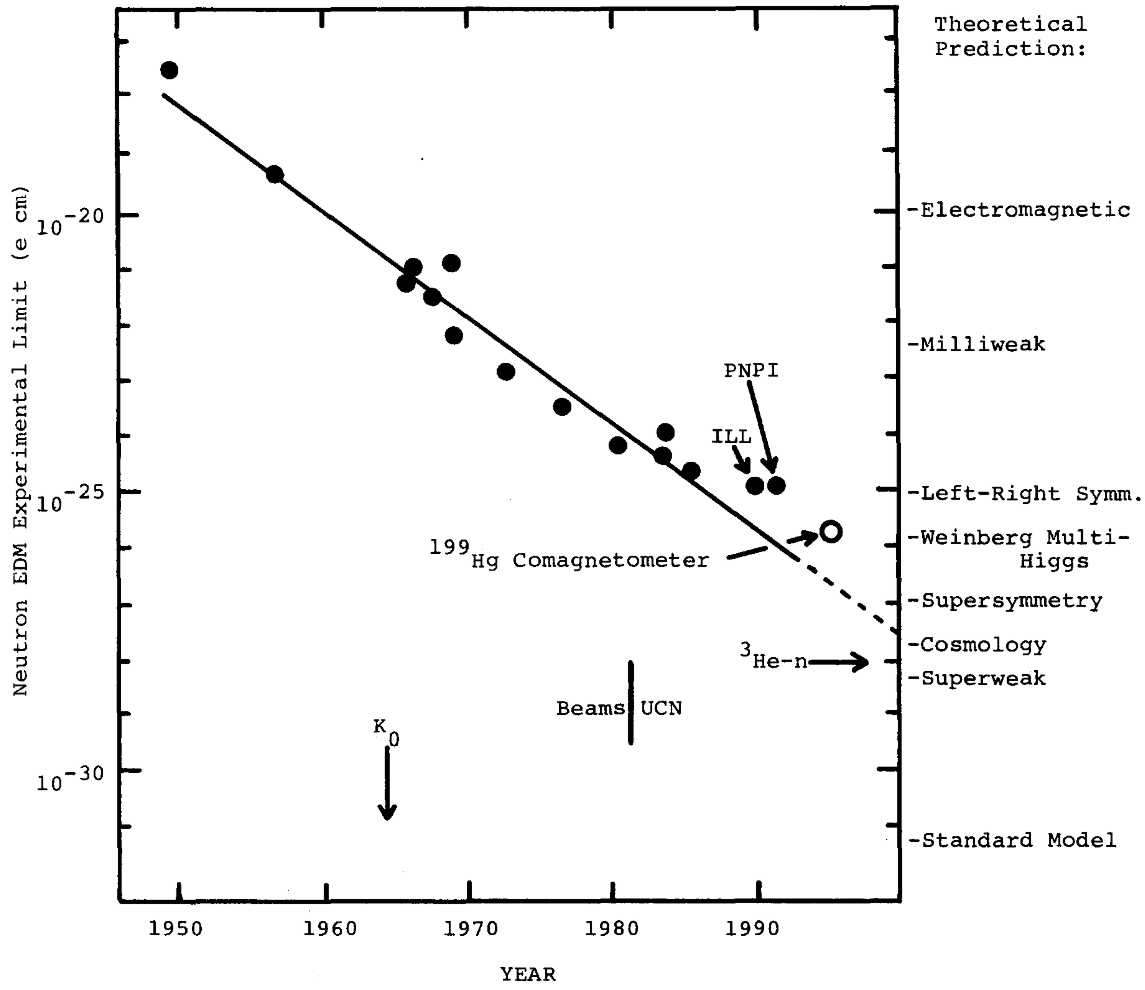
\includegraphics[width=\textwidth]{img/history_of_nedm_measurements}
	\caption{Measurement history of the neutron EDM \cite{Golub1994}}
	\label{fig:edm_history}
\end{figure}

Hopefully these reasons would convince even the most demanding reader in the need to conduct the n2EDM experiment. But what is \textit{n2EDM} exactly? We will try to explain that in the next chapter.

\chapter{The n2EDM experiment}
\label{chapter:experiment}

Knowledge is power and our knowledge of the physical property that can be measured to show the violation of the \textit{CP}-symmetry is an important first step in solving the riddle of the baryogenesis. Now we just need to get our hands dirty with some experimental data. It will be obtained over the course of the n2EDM experiment currently being built at PSI (Paul Scherrer Institute, Villigen, Switzerland).

\textit{What will be measured?} Electric dipole moment of the neutron. The neutrons were chosen for the following reasons:
\begin{itemize}
	\item They are electrically neutral\footnote{Which is quite important for an experiment based in Switzerland}, which means that they would not be dragged by the electric field $\vec{E}$
	\item There are nuclear reactions that allow to produce them efficiently, like fission or spallation (which is already available in PSI and will be used)
	\item They can be cooled down to become UCNs (ultracold neutrons)
\end{itemize}

\textit{What are ultracold neutrons and why do we like them?} We call \cite{Fermi1936} a neutron ultracold when it has a kinetic energy $E_{kin} \leq 300\ \text{neV}$. Such low energy brings the following experimental benefits:
\begin{itemize}
	\item Ease of collection, since the neutrons would behave similar to ping-pong balls, bouncing from the surface of a neutron vessel.
	\item Possibility to store \cite{Zeldovich1959} the neutrons up to their lifetime of $\approx 886\ \text{s}$ \cite{Tanabashi2018}.
	\item Weakening of a so-called $\vec{v} \times \vec{E}$ effect \cite{Pendlebury2004}, which arises from the coupling of a particle spin $\vec{I}$ itself with an electric field $\vec{E}$. This would bring the effective Hamiltonian closer to one mentioned in Eq. \ref{eq:neutron_hamiltonian}.
\end{itemize}

\textit{What precision do we expect?} By using only the Standard Model it is possible to get an estimation \cite{Khriplovich1982} of the neutron EDM at the following level:
\begin{equation}
	d_n \approx 2 \cdot 10^{-32}\ e \cdot \text{cm}
\end{equation}

The \textbf{n2EDM} experiment is conceptually following the footsteps of the results obtained by the \textbf{nEDM} collaboration. By analysing the data obtained at ILL, Grenoble it was possible to achieve \cite{Pendlebury2015} an impressive record of $d_n$ precision:
\begin{equation}
	\left| d_n \right| < 3.6 \cdot 10^{-26}\ e \cdot \text{cm (95\% CL)}.
\end{equation}

This leaves us with 6 more orders of magnitude to go. The n2EDM experiment aims to cut this number to five, improving \cite{Abel2018} the precision tenfold.

\textit{What method will be used?} Same as in the original nEDM experiment, Ramsey method of the time separated oscillating fields.%
\begin{figure}[h]
	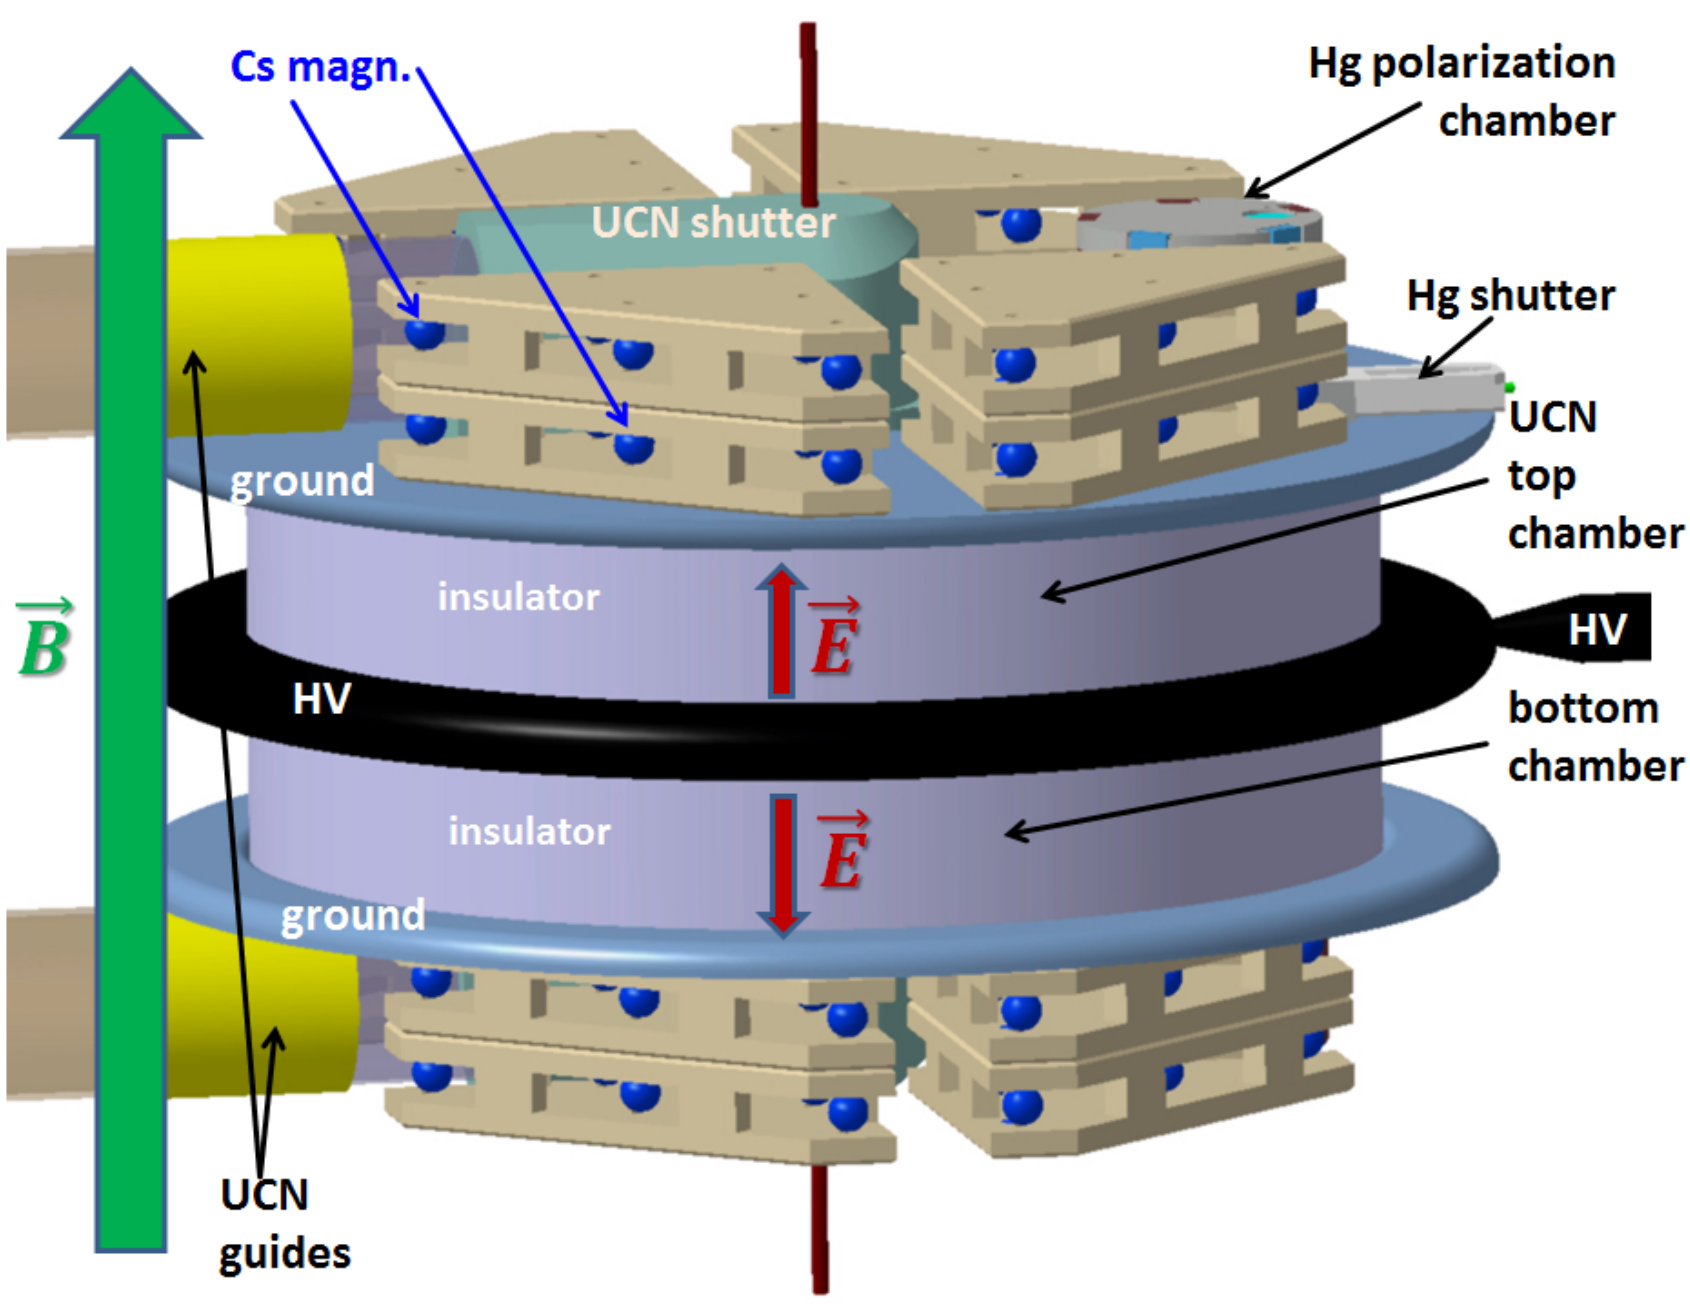
\includegraphics[width=\textwidth]{img/n2edm_chamber}
	\caption{Double chamber design \cite{Abel2018}.}
	\label{fig:precession_chamber}
\end{figure}

One can see that the precession chamber pictured in the Fig. \ref{fig:precession_chamber} features fields $\vec{E}$ and $\vec{B}$ that are codirectional in one chamber and contradirectional in another. In both chambers the neutron can be described with the Hamiltonian from Eq. \ref{eq:neutron_hamiltonian}. Let's take a look at its Larmor precession.

In the case of the \textbf{codirectional} fields we can write
\begin{equation}
	h\nu_{\uparrow \uparrow} = -2 \left( \mu_n B_{\uparrow \uparrow} + d_n E_{\uparrow \uparrow} \right).
	\label{eq:larmor_codirectional}
\end{equation}

If the fields are \textbf{contradirectional} we will get
\begin{equation}
	h\nu_{\uparrow \downarrow} = -2 \left( \mu_n B_{\uparrow \downarrow} - d_n E_{\uparrow \downarrow} \right).
	\label{eq:larmor_contradirectional}
\end{equation}

By combining Eq. \ref{eq:larmor_codirectional} and Eq. \ref{eq:larmor_contradirectional} we can express the neutron electric dipole moment $d_n$ through the fields $E$ and $B$, magnetic moment $\mu_n$ and Larmor frequencies $\nu_{\uparrow \uparrow}$ and $\nu_{\uparrow \downarrow}$ as
\begin{equation}
	d_n = \frac{h \left( \nu_{\uparrow \downarrow} - \nu_{\uparrow \uparrow} \right) - 2 \mu_n \left( B_{\uparrow \uparrow} - B_{\uparrow \downarrow} \right)}{2 \left( E_{\uparrow \uparrow} + E_{\uparrow \downarrow} \right)}.
\end{equation}

\textit{Why is the double chamber design important?} The idea of a double chamber pioneered \cite{Altarev1980} in 1980. The biggest improvement that it brings is the ability to measure the Larmor frequency for the codirectional and the contradirectional cases \textbf{simultaneously}. This feature allows to strongly reduce \cite{Abel2018} any time dependent systematic effects.

\textit{How does n2EDM look like schematically?} You can see it on the Fig. \ref{fig:n2edm_schema}.%
\begin{figure}[h]
	\centering
	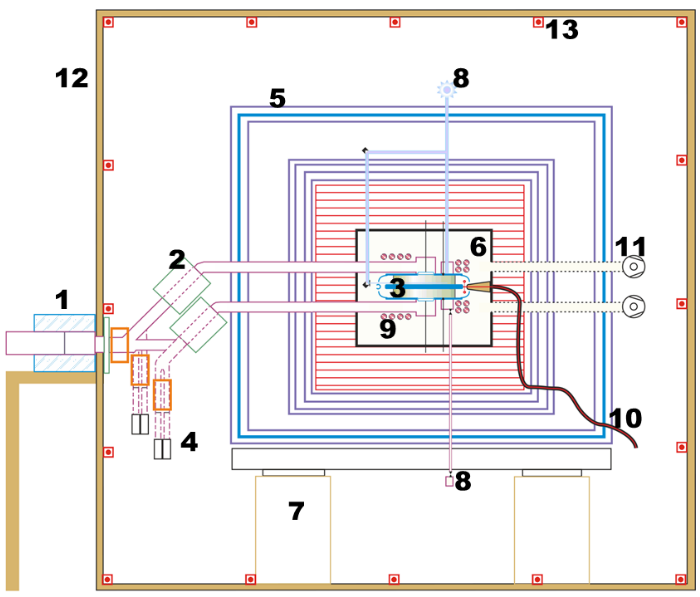
\includegraphics[width=.82\textwidth]{img/n2edm_schema}
	\caption{Schema of the experimental setup \cite{Abel2018}.}
	\label{fig:n2edm_schema}
\end{figure}

It features \cite{Abel2018} the following:
\begin{enumerate}
	\item A $5\ \text{T}$ superconductive polarizer magnet to align the spin of UCNs before they enter precession chambers
	\item Switches to control the filling and emptying of the UCN chambers
	\item Two precession chambers, portrayed in details on Fig. \ref{fig:precession_chamber}
	\item Four spin projection detectors --- for every chamber we count amount of neutrons with spins up and down
	\item Magnetically shielded room to protect the storage chambers and the vacuum vessel
	\item The vacuum vessel
	\item Four granite pillars supporting an $Al$ plate
	\item The $Hg$ magnetometer to measure the average magnetic fields
	\item The $Cs$ magnetometer to measure the gradients of the magnetic field
	\item A high voltage cable
	\item The molecular pumps generating vacuum in the vacuum vessel
	\item Insulation shell, thermally stabilized by air-conditioning (not shown)
	\item Surrounding field compensation (SFC) system is designed to actively minimise the magnetic perturbations of the environment
\end{enumerate}

\begin{figure}[h]
	\centering
	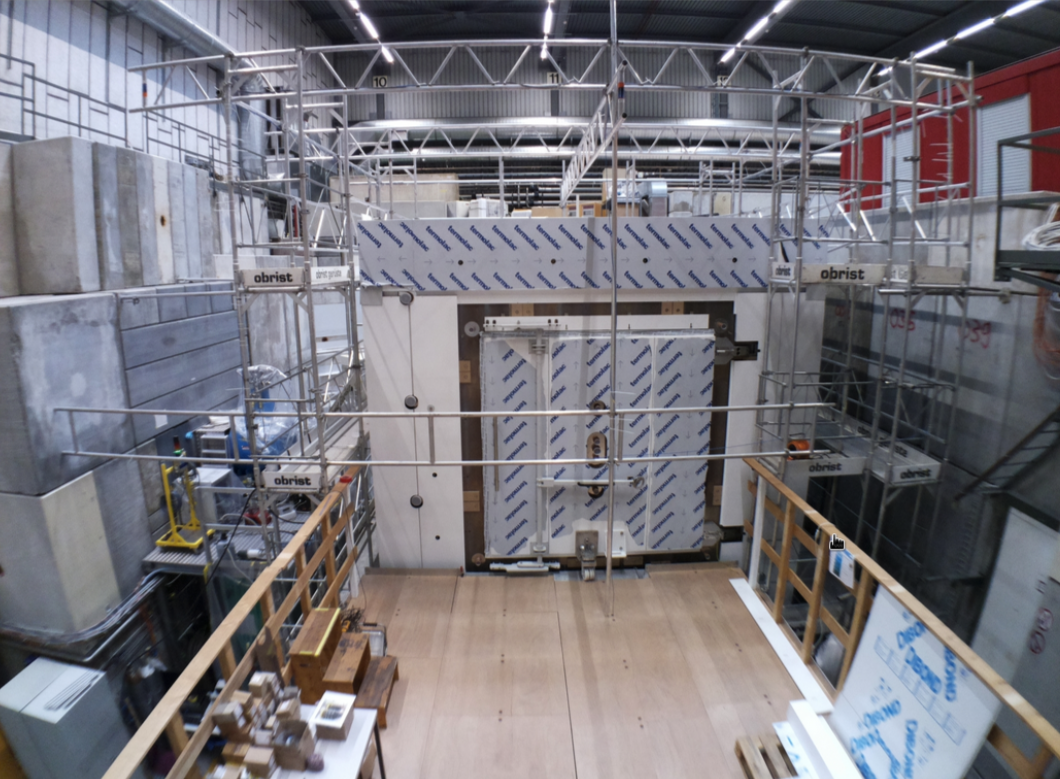
\includegraphics[width=.86\textwidth]{img/n2edm_photo}
	\caption{Recent photo of the n2EDM experiment \cite{Germann2019}.}
	\label{fig:n2edm_photo}
\end{figure}%
\textit{How does n2EDM actually look at the moment?} Like it is shown on the Fig. \ref{fig:n2edm_photo}.%
\chapter{The n2EDM DAQ system}
\label{chapter:daq}

In order to measure the neutron EDM and question the theoretical predictions mentioned in the Chapter \ref{chapter:introduction} it is not enough to do a single cycle of the experimental setup from the Chapter \ref{chapter:experiment}. Everything comes at a price and pushing the limits of precision is not an exception. The analysis \cite{Pendlebury2004} of the previous nEDM experiment was based on data collected between 1998 and 2002, with each data-taking run lasting about 1--2 days. Thus a solid and performant data acquisition and control (DAQ) system is strongly needed.

\textit{Why cannot we just reuse the DAQ from nEDM?} Apart from an experimental setup containing new modules and equipment there are \cite{Bison2018} other reasons for us to consider designing a new generation of the DAQ system:

\begin{itemize}
	\item Complexity of the codebase (one of the projects consisted of approximately 748\,332 LabView VIs) was limiting modifications
	\item Inability to test or debug the DAQ system without the complete experimental environment, including the hardware, being connected. This was blocking data acquisition or the regular shift routine
	\item No standardisation in connecting various hardware devices to the DAQ, resulting in the code repetition
	\item Windows operating system lock-in
\end{itemize}

\textit{What principles is the n2EDM DAQ built on?} The new \textbf{n2EDM} DAQ aims to address the main pain points and limitations of the old \textbf{nEDM} DAQ by selecting to follow the design ideas listed below:

\begin{itemize}
	\item \textbf{TCP/IP communication}: by relying on the TCP/IP as the transport layer we can guarantee deliverability of messages in the same order as they were sent. By being an industrial standard it also simplifies connection of the new hardware nodes to the system. Not specifically TCP/IP-related bonus is that by optically decoupling our hardware it is possible to automatically provide electrical insulation
	\item \textbf{SCPI syntax}: all commands should be written following a human-readable specification \cite{SCPIConsortium1999}. This would standardise the environment and allow for the simpler debugging
	\item \textbf{Script control}: what can be better than a single SCPI command? Only a human-readable repeatable set of commands, providing an ability to program the behaviour of the experimental setup
	\item \textbf{Modularity}: usage of the small loosely connected independent modules improves robustness and encourages testing. Additionally if modules can be tested without the presence of each other it also becomes simpler to implement the End-to-End (E2E) testing of the whole system with the aim of being able to arbitrary replace physical equipment with its software-only analogs. This brings us closer to an ability to run the n2EDM experiment in a simulation mode
	\item \textbf{Linux based}: apart from being free (both as in "free as a speech" and "free as a beer") the development ecosystem of Linux provides much more opportunities compared to the Windows one. Even though the recent release \cite{Loewen2019} of the Windows Subsystem for Linux made the difference less painful, one might still prefer to run the programs directly on Linux with zero overhead
\end{itemize}

\begin{figure}[h]
	\centering
	\includegraphics[width=\textwidth]{img/daq_schema.png}
	\caption{Schematic view of the n2EDM DAQ system. Based on \cite{Bison2018}.}
	\label{fig:daq_schema}
\end{figure}

Let's take a closer look at some of the core components of the n2EDM DAQ system presented on the Fig. \ref{fig:daq_schema}.

\section{Command Distributor}
\label{sec:distributor}

\url{https://gitlab.com/n2edm/n2sim}

The distributor acts like a spinal cord of the system, combining the functions of the message bus and the modules registry. Every node registers itself with the distributor by providing its name, upstream and downstream FIFOs. For example, the GUI node might provide the following information to the distributor:

\begin{itemize}
	\item \textbf{Module name}: \texttt{GUI}
	\item \textbf{Upstream file}: \texttt{/n2edm/fifos/\_GUI\_upstream}
	\item \textbf{Downstream file}: \texttt{/n2edm/fifos/\_GUI\_downstream}
\end{itemize}

Now another node wants to communicate with the GUI node. To do that it would send \texttt{GUI:COMMAND} to the distributor. Distributor would check whether the module with name \texttt{GUI} has been registered. If this is the case the message would be forwarded to the appropriate FIFO, in our example that would be \texttt{/n2edm/fifos/\_GUI\_downstream}.

Direct communication with the distributor is possible by writing into a hardcoded path \texttt{/n2edm/\_n2sim\_input}. User can simulate the behaviour described above by executing this command:
\begin{verbatim}
	echo "GUI:COMMAND" >> /n2edm/_n2sim_input
\end{verbatim}

\section{Dispatcher}
\label{sec:dispatcher}

\url{https://gitlab.com/n2edm/n2dispatcher}

The dispatcher provides a generic mechanism for executing commands on the central server. It should be enough to have the distributor and the dispatcher running to boot up every other module located on the same computer. One could imagine the following flow:
\begin{enumerate}
	\item Content of the repository \url{https://gitlab.com/n2edm/startscripts} is cloned into the \texttt{/n2edm/startable} folder of the central server
	\item Scripts in this folder are made executable
	\item Distributor and dispatcher are started
	\item User sends \texttt{n2dispatcher:startch 'runcyclenumber',''} to the distributor
	\item Dispatcher executes \texttt{/n2edm/startable/runcyclenumber} and starts the run \& cycle manager
\end{enumerate}

Dispatcher is also reachable directly via TCP/IP. A possible scenario could be that the remote node boots up and asks the dispatcher to start a corresponding COM handler. This way this node would become included into the global communication system.

\section{Run \& Cycle Manager}
\label{sec:runcyclemanager}

\url{https://gitlab.com/n2edm/runcyclenumber}

This node records and distributes to other nodes information from the UCN source about the run and cycle number. This is needed to be able to store and analyse experimental data. Every node that writes binary data to disk uses this information for the distinguishable file names.

\section{Data Storage}
\label{sec:data_storage}

Since it is expected for the n2EDM experiment to generate loads of data it is absolutely necessary to preserve it for the further analysis. Initially data is written to the disk of the central server, however most likely it would not be able to fit the whole volume generated over 5--10 years, thus demanding a secondary larger storage. In order to simplify data management and avoid conflicts of the file versions information from the Run \& Cycle Manager is used to transfer the files only after being completed. These static data samples would be distributed further among the partner universities and additional backups. However some nodes, like a GUI node, would need the data accessible in a nearly real-time mode. For that purpose a volatile copy of the most recent files would be provided with the expected delay being below 10 seconds.

\section{Timing Infrastructure}
\label{sec:timing_infrastructure}

One of the principal positions \cite{Bison2018} of the n2EDM experiment is synchronous equidistant data sampling. We introduce a heartbeat sampling rate of 10 Hz meaning that every node must write its current state to the disk every $1/10$ second and every node need to do it at the same absolute time as all other nodes. In other words, we want to be able to describe the joint state of the system 10 times per second. This approach helps to study systematic uncertainties, eases the correction of correlations and additionally enables us to represent the state evolution as a (FFT) spectrum or as an Allan deviation to simplify the data analysis.

This requires all nodes to have their time synchronised between each other. We solve it by using a central GPS controlled grandmaster clock which provides time to the nodes via the precision time protocol (PTP). The accuracy guaranteed by the PTP should be enough for the most tasks, however some systems, like the Accurate Frequency Unit from the Fig. \ref{fig:daq_schema} additionally use the dedicated 10 MHz lines to further improve synchronisation veracity.

\section{COM Handler}
\label{sec:com_handler}

\url{https://gitlab.com/n2edm/n2comhandler}

In order to connect the remote nodes to the distributor we need to utilise their TCP/IP endpoint and stitch it together with the corresponding POSIX pipes. COM handler is a smart bridge that does that and additionally provides the following features:

\begin{itemize}
	\item Auto-registers itself with the distributor
	\item Buffers the commands if the node is unavailable
	\item Allows to use the response of the node by other components via a generic \texttt{REPLYTO} command
	\item Handles generation of the header and data files by using information from the run \& cycle manager
\end{itemize}

As one can see, the COM handler is one of the essential parts of the n2EDM DAQ system and thus it demands a special attention to the design details.

\section{Sequencer}
\label{sec:sequencer}

\url{https://gitlab.com/n2edm/sequencer}

In order to program the DAQ system one needs a programming language and an environment that supports it. Sequencer provides the latter and aims to support a set of basic coding blocks that is flexible enough to describe arbitrary behaviour of the individual nodes and system as a whole:

\begin{itemize}
	\item \textbf{Conditionals}: \texttt{IF (...) THEN ... ELSE ... ENDIF}
	\item \textbf{Cycles}: \texttt{FOR (...) DO ... DONE}
	\item \textbf{Variables (local value)}: \texttt{SET variable = expression}
	\item \textbf{Variables (remote value)}: \texttt{SET variable = REQUEST(...)}
	\item \textbf{Direct source manipulation}: \texttt{(ADD/INSERT/REPLACE/DELETE)LINE}
	\item \textbf{Navigation}: \texttt{LABEL "..."} and \texttt{GOTO "..."}
	\item \textbf{Lifecycle management}: \texttt{SLEEP ...s}, \texttt{PAUSE}, \texttt{RESUME}
\end{itemize}

The list above is non-exhaustive but nevertheless gives an impression of how one can control the n2EDM DAQ system. A more detailed explanation of the role and the capabilities of the sequencer can be found in \cite{Germann2019}.






















\chapter{Features}
\label{chapter:features}

Now that we have an understanding about the way the n2EDM DAQ system is expected to operate we can shift the focus of our discussion to the work that was conducted over the course of this thesis. In this chapter we will explain the way they were designed and implemented, additionally highlighting their capabilities as well as the limitations the future developers and/or users might face.

\section{Support of the \texttt{FOR} loop}
\label{sec:for_loop}

\textit{Components affected}: \textbf{Sequencer} (Section \ref{sec:sequencer}).

\textit{Motivation}: While the sequencer is able to execute the pseudo-\texttt{FOR} loop as shown on the Listing \ref{listing:goto_as_for} we would still prefer to have it implemented as a standalone construction for the sake of simplicity and reducing the mental overhead of the users. Additionally the usage of \texttt{GOTO} command is generally considered \cite{Dijkstra1968} harmful, leading to the unstructured spaghetti code \cite{Cram2005}.

\begin{lstlisting}[
	caption={Implementing \texttt{FOR} with \texttt{GOTO}}, 
	label={listing:goto_as_for}, 
	language=n2EDMScript
]
SET i = 0
LABEL "FOR_START"
IF $i < 5 THEN
...
SET i = $i + 1
GOTO "FOR_START"
ELSE
ENDIF
\end{lstlisting}

\textit{Requirements}: We introduce 3 new commands that the sequencer should be able to handle:

\begin{itemize}
	\item \texttt{FOR (init; test; iterate)} or \texttt{FOR ((init; test; iterate))}. Amount of whitespace characters is arbitrary, round brackets are allowed as a part of every argument, but amount of \colorbox{selectioncolor}{\strut \texttt{(}} and \colorbox{selectioncolor}{\strut \texttt{)}} per argument needs to be balanced. Nested \texttt{FOR} blocks are allowed.
	\begin{itemize}
		\item \texttt{init}: an expression that is being executed once to init the state of the loop variable. It follows the semantic of the \texttt{SET} operator, for example \texttt{i = 0} is valid.
		\item \texttt{test}: an expression that produces a boolean value when evaluated. We run this check on every iteration, including the first one. Semantically similar to the argument of the \texttt{IF} block, so \texttt{\$i < 5} is allowed. If the output is \texttt{False}, skipping the lines until a \texttt{DONE} block is encountered. Otherwise continues execution as usual.
		\item \texttt{iterate}: an expression that is used to modify the loop variable. Gets evaluated at the end of every cycle. It borrows the structure of the \texttt{SET} command, usually using the loop variable itself in a following manner: \texttt{i = \$i + 1}
	\end{itemize}
	\item \texttt{DO}: contrary to the name it does nothing. If encountered, must have a valid \texttt{FOR} statement in a previous line of the sequence.
	\item \texttt{DONE}: marks the end of the \texttt{FOR} loop. Redirects to the beginning of the loop for the next iteration.
\end{itemize}

We should be able to replace the Listing \ref{listing:goto_as_for} with the code of the Listing \ref{listing:for_loop_example}.
\begin{lstlisting}[
	caption={Example of the \texttt{FOR} loop}, 
	label={listing:for_loop_example},
	language=n2EDMScript
]
FOR (i = 0; $i < 5; i = $i + 1)
DO
...
DONE
\end{lstlisting}

\textit{Implementation details}: 

\begin{itemize}
	\item Contrary to the implementation of the \texttt{IF/ELSE/ENDIF} blocks the \texttt{FOR} loop does not need to be complete all the times. Rather if we encounter \texttt{FOR} we evaluate the \texttt{FOR.test} condition and continue executing or skipping the next lines based on the condition's output until the matching \texttt{DONE} is found
	\item Current scope of the variables is always global, so one might prefer to use different iteration variables for nested loops to prevent confusing results
	\item Sequencer supports powerful inline editing/removal of the lines. We do not attempt to prevent cases like \texttt{GOTO} from the loop body or \texttt{REMOVELINE} of \texttt{FOR} while iterating. However the sequencer will always try to find the root of the problem and notify the user about it
	\item Default strategy for the non-parseable lines is to skip them
\end{itemize}

%\begin{lstlisting}[
%	language=JavaScript, 
%	caption={Simplified overview of the \texttt{FOR} loop implementation},
%	label={listing:for_loop_implementation}
%]
%let skipUntilDone = false
%let forDelta = 0
%
%while (canReadNextSequenceLine) {
%	++currentLineNumber
%
%	if (skipUntilDone) {
%		if (isCurrentLine('FOR')) {
%			++forDelta
%		} else if (isCurrentLine('DONE')) {
%			--forDelta
%
%			if (forDelta == 0) {
%				skipUntilDone = false
%			}
%		}
%	} else if (isCurrentLine('FOR')) {
%		setVariable(forLine.init)
%		skipUntilDone = !evaluateExpression(forLine.test)
%
%		if (skipUntilDone) {
%			forDelta = 1
%		}
%	} else if (isCurrentLine('DO')) {
%		const savedCurrentLineNumber = currentLineNumber
%		let doneDelta = 1
%
%		do {
%			--currentLineNumber
%			if (isCurrentLine('FOR')) {
%				--doneDelta
%			} else if (isCurrentLine('DONE')) {
%				++doneDelta
%			}
%		} while (!(doneDelta == 0 || currentLineNumber == 0))
%
%		if (doneDelta != 0) {
%			currentLineNumber = savedCurrentLineNumber
%		} else {
%			setVariable(forLine.iterate)
%			const canRunAgain = evaluateExpression(forLine.test)
%
%			if (!canRunAgain) {
%				currentLineNumber = savedCurrentLineNumber
%			}
%		}
%	}
%}
%\end{lstlisting}
\newpage
\section{Improved the \texttt{REQUEST} command}
\label{sec:request}

\textit{Components affected}: \textbf{Sequencer} (Section \ref{sec:sequencer}).

\textit{Motivation}: while the core functionality of this feature was provided by \cite{Germann2019} the implementation contained a few undesired restrictions:

\begin{itemize}
	\item At any given moment of time only 1 request could have been pending
	\item In order to pause the execution while request was in flight, functionality of \texttt{SLEEP} command was used. This would have lead to unexpected results when combining \texttt{SLEEP}, \texttt{PAUSE}, \texttt{RESUME} and \texttt{REQUEST} blocks.
	\item Without the Feature \ref{sec:replyto} it could have not been tested thoroughly and contained a number of bugs.
\end{itemize}

\textit{Requirements}: sequencer needs to support the \texttt{SET variable = REQUEST( question, format, timeout, default)} instruction with the semantics as described below:

\begin{itemize}
	\item \texttt{question}: required quoted string starting with \highlight{:}. Represents the node name and the  command that should return the value that we are interested in. Example: \texttt{":HV:OUTPUT:VOLTAGE?"}.
	\item \texttt{format}: optional string (\texttt{\%0} if not provided). In case the target node returns multiple comma-separated values this argument in the form of \texttt{\%n} selects the n-th element starting with 1. Special case \texttt{\%0} instructs to return the node response as a whole.
	\item \texttt{timeout}: optional int/double (\texttt{1} if not provided). Maximum amount of seconds the sequencer needs to wait for the answer.
	\item \texttt{default}: optional int/double (\texttt{0} if not provided). The value used in case the request does not return an answer within the \texttt{REQUEST.timeout}.
\end{itemize}

First step in getting the answer is sending the request itself. Let's discuss how every \texttt{REQUEST} statement should be processed before getting sent to the distributor. \texttt{REQUEST(":HV:OUTPUT:VOLTAGE?", \%2, 1, 0)} would serve us as an example:

\begin{enumerate}
	\item We select the \texttt{nodeName} from the \texttt{REQUEST.question}, in our case it would be the \texttt{:HV}, leaving \texttt{:OUTPUT:VOLTAGE?} as a \texttt{nodeCommand}
	\item{
		We create a quoted \texttt{argumentsString} which looks like 
		\begin{verbatim}
			"sequencerNodeName:RESULT requestId, REQUEST.format"
		\end{verbatim}
		\begin{itemize}
			\item \texttt{sequencerNodeName} is the name with which the sequencer was registered with the distributor, let's assume it is \texttt{SEQUENCER}.
			\item \texttt{requestId} is a unique positive integer used to distinguish the received answers, we would select 17.
		\end{itemize}
		In our case \texttt{argumentsString} would be \texttt{"SEQUENCER:RESULT 17, \%2"}
	}
	\item{
		We create a final \texttt{requestCommand} of the shape
		\begin{verbatim}
			nodeName:REPLYTO(argumentsString)nodeCommand
		\end{verbatim}
		or for the example that we have started with
		\begin{verbatim}
			HV:REPLYTO("SEQUENCER:RESULT 17, %2"):OUTPUT:VOLTAGE?
		\end{verbatim}
	}
	\item The \texttt{requestCommand} is sent to the distributor.
\end{enumerate}

Second step is receiving the answer. To do that, sequencer supports the \texttt{RESULT} command. Following the example we expect to receive a string \texttt{RESULT 17, remoteValue} and execute \texttt{SET variable = remoteValue}. One could notice that the node answer looks like if the \texttt{argumentsString} from above would have been used as a template.

Sequencer supports 2 sources of commands, called external and internal. External commands are the one that arrive from the distributor. Internal commands come from a sequence of commands that the sequencer stores in memory. A command can be loaded into this sequence from the external commands, for example with \texttt{ADDLINE "..."}. For this feature we are only interested in a subset of commands from both sides:

\begin{itemize}
	\item \textbf{External}:
	\begin{itemize}
		\item \texttt{PAUSE}. Pauses the execution of all internal commands until the \texttt{RESUME} is received.
		\item \texttt{RESUME}. Resumes the execution of all internal commands if paused by \texttt{PAUSE}.
		\item \texttt{RESTART}. New command, removes information about all requests, rewinds the internal sequence to the first line, cancels any blocks introduced by \texttt{PAUSE} or \texttt{SLEEP}. \textbf{Preserves} the state of all variables.
		\item \texttt{SET variable = REQUEST(...)}. Pauses the execution of the internal commands until either an answer is returned or the timeout of the corresponding request was reached, whatever event happens earlier. Sets the variable to the received or default value.
	\end{itemize}
	\item \textbf{Internal}:
	\begin{itemize}
		\item \texttt{SLEEP ...s}. Pauses the execution of the internal sequence for a given amount of seconds. Is \textbf{not} equal to pausing the sequencer with \texttt{PAUSE}.
		\item \texttt{SET variable = REQUEST(...)}. Same logic as if it would have been executed directly from the external source.
	\end{itemize}
\end{itemize}

\newpage

\textit{Implementation details}:

\begin{itemize}
	\item{
		The execution of the internal sequence can be paused independently by multiple events:
		\begin{enumerate}
			\item \texttt{PAUSE} and reaching the end of the sequence set the internal \texttt{isPaused} flag to \texttt{True}.
			\item \texttt{SLEEP} sets the \texttt{isSleeping} flag to \texttt{True} and saves the time at which it should be set back to \texttt{False}.
			\item At least 1 pending request is in flight.
		\end{enumerate}
		The execution continues only in case of none of these blocking conditions being present.
	}
	\item{
		A somewhat unexpected consequence of sharing the \texttt{SET} logic is that the \texttt{REQUEST} can be also used as part of the Feature \ref{sec:for_loop}. Both \texttt{FOR.init} and \texttt{FOR.iterate} can be \texttt{REQUEST}ed, making the following line valid:
\begin{lstlisting}[language=n2EDMScript, numbers=none]
FOR (i = REQUEST(...); $i < 5; i = REQUEST(...))
\end{lstlisting}
	}
\end{itemize}

%In the Listing \ref{listing:request} we present a skeleton that handles the sending/receival of the requests as well as the management of the execution state.

%\begin{lstlisting}[
%	language=JavaScript,
%	caption={Simplified overview of the \texttt{REQUEST} command implementation},
%	label={listing:request}
%]
%interface RequestMetadata {
%	id: number
%	isActive: boolean
%	variableName: string
%	defaultValue: string
%	start: Date
%	deadline: Date
%}
%
%const requests = new Map<number, RequestMetadata>()
%let currentRequestId = 1
%
%function getPendingRequests() {
%	const result: RequestMetadata[] = []
%
%	for (const request of requests.values()) {
%		if (request.isActive) {
%			result.push(request)
%		}
%	}
%
%	return result
%}
%
%function areRequestsPending() {
%	const pendingRequests = getPendingRequests()
%
%	if (pendingRequests.length > 0) {
%		return true
%	} else {
%		return false
%	}
%}
%
%function cleanRequests() {
%	requests.clear()
%}
%
%function sendRequestToDistributor(
%	question: string,
%	format: string,
%	timeout: string,
%	defaultValue: string,
%	variableName: string
%) {
%	++currentRequestId
%
%	const command = createReplyToCommand(
%		question,
%		currentRequestId,
%		format,
%		defaultValue
%	)
%
%	const deadline = addSeconds(new Date(), timeout)
%	requests.set(currentRequestId, {
%		id: currentRequestId,
%		isActive: true,
%		variableName,
%		defaultValue,
%		start: new Date(),
%		deadline
%	})
%
%	sendCommand(command)
%}
%
%function handleDistributorResponse(
%	responseId: number, 
%	responseValue: string
%) {
%	const request = requests.get(responseId)
%
%	if (new Date() > request.deadline) {
%		requests.delete(responseId)
%		return
%	}
%
%	setVariable(request.variableName, responseValue)
%	requests.delete(responseId)
%}
%
%function checkRequestTimeout() {
%	const pendingRequests = getPendingRequests()
%
%	for (const request of pendingRequests) {
%		if (new Date() > request.deadline) {
%			setVariable(request.variableName, request.defaultValue)
%			request.isActive = false
%		}
%	}
%}
%
%function setVariable(expression: string) {
%	if (isCommand(expression, 'REQUEST')) {
%		sendRequestToDistributor(
%			question,
%			format,
%			timeout,
%			defaultValue,
%			variableName
%		)
%	}
%}
%
%let isPaused = true
%let isSleeping = false
%let endOfSleep = new Date()
%
%function analyse(command: string) {
%	if (isCommand(command, 'PAUSE')) {
%		isPaused = true
%	} else if (isCommand(command, 'RESUME')) {
%		isPaused = false
%	} else if (isCommand(command, 'RESTART')) {
%		isPaused = false
%		isSleeping = false
%		currentLineNumber = 0
%		cleanRequests()
%	} else if (isCommand(command, 'SET')) {
%		setVariable(command)
%	} else if (isCommand(command, 'RESULT')) {
%		handleDistributorResponse(responseId, responseValue)
%	}
%}
%
%function resume() {
%	const blockedByRequests = areRequestsPending()
%
%	if (!isPaused && !isSleeping && !blockedByRequests) {
%		if (!canReadNextSequenceLine) {
%			isPaused = true
%		} else {
%			++currentLineNumber
%
%			if (isCurrentLine('SLEEP')) {
%				endOfSleep = addSeconds(new Date(), seconds)
%			} else if (isCurrentLine('SET')) {
%				setVariable(expression)
%			}
%		}
%	}
%
%	if (isSleeping) {
%		if (new Date() > endOfSleep) {
%			isSleeping = false
%		}
%	}
%
%	if (blockedByRequests) {
%		checkRequestTimeout()
%	}
%}
%
%while (!shouldExit) {
%	const command = readOneExternalCommand()
%
%	if (command.length > 0) {
%		analyse(command)
%	} else {
%		resume()
%	}
%}
%\end{lstlisting}

\section{Implemented the \texttt{REPLYTO} command}
\label{sec:replyto}

\textit{Components affected}: \textbf{COM Handler} (Section \ref{sec:com_handler})

\textit{Motivation}: in order to create a truly interconnected DAQ system it is not enough to be able to send SCPI commands to our nodes. We also need to be able to use their responses for a feedback loop of any kind. By implementing this feature on the COM handler level it  would be possible to return a response of any node.

\textit{Requirements}: following the contract of the \texttt{REQUEST} Feature \ref{sec:request} the COM handler needs to support a \texttt{:REPLYTO} command. We would like to achieve a behaviour as described below:

\begin{itemize}
	\item Only one \texttt{:REPLYTO} command can be processed at a time. When it is executed the COM handler should continue accepting commands from the distributor. These commands would be buffered in memory until the pending \texttt{:REPLYTO} command completes.
	\item{
		Given the example from the Feature \ref{sec:request}
		\begin{verbatim}
			HV:REPLYTO("SEQUENCER:RESULT 17, %2"):OUTPUT:VOLTAGE?
		\end{verbatim}
		we will send \texttt{OUTPUT:VOLTAGE?} to the node and pause the further execution of the SCPI commands.
	}
	\item{
		Upon executing the \texttt{:REPLYTO} command the COM handler sets a time window based on the integer \texttt{scpiResponseTimeoutMs} value from the config file \texttt{conf\_n2comhandler.cfg}. We have 3 cases to handle:
		\begin{itemize}
			\item If nothing came over the SCPI connection with the node during the waiting interval then it means that \texttt{:REPLYTO} has timed out. We resume the execution of the SCPI commands from the distributor from the next command, if any.
			\item If a complete message that starts with \highlight{:} was received then we assume that the node is trying to communicate with other components of the system. Such message is forwarded to the distributor directly as is and does not influence the \texttt{:REPLYTO} feature flow.
			\item Otherwise if a complete message was received while we are still within the time window of waiting for response then we consider it to be an answer to the \texttt{:REPLYTO} being in flight.
			\item If a node answer that does not start with \highlight{:} was received outside of the \texttt{:REPLYTO} timeout the COM handler would skip it and print a warning.
		\end{itemize}
		\item{
			If a complete SCPI response was received in time then our next task is to parse it. A node might decide to return multiple comma-separated values. We split the message into chunks by using the rules below:
			\begin{itemize}
				\item Message is scanned from left to right
				\item Splittable parts are separated by commas \highlight{,}
				\item Escaped commas \highlight{\textbackslash ,} are not separators
				\item Commas that appear inside of a string are not separators
				\item String starts with a quotation mark \highlight{"}
				\item String might end with a quotation mark \highlight{"}. If there is no closing quotation mark, we consider the string to end at the end of the message. So in \texttt{"1,2,3} none of the commas would be a separator
				\item Escaped quotation marks \highlight{\textbackslash "} are not considered quotation marks
			\end{itemize}
		}
		\item{
			After splitting the message we need to extract the correct \texttt{answerValue} by using the format argument, in our example that would be \texttt{\%2}
			\begin{itemize}
				\item \texttt{\%0} means that no splitting is required and \texttt{answerValue} is set to the received message as a whole
				\item \texttt{\%n} means that \texttt{answerValue} is set to the \texttt{n}-th part of the split message with count starting with 1. If the message contained no separators then \texttt{\%0} and \texttt{\%1} produce the equal output. If the split message contains less than \texttt{n} parts we set \texttt{answerValue} to an empty unquoted string.
			\end{itemize}
		}
		\item After extracting the \texttt{answerValue} we are ready to send back the answer. Let's assume that \texttt{answerValue = 289}. Following our example, the COM handler will need to send \texttt{:SEQUENCER:RESULT 17, 289} over FIFO to the distributor.
	}
\end{itemize}

\textit{Implementation details}:

\begin{itemize}
	\item{
		In the \textit{requirements} above one can often see a combination of words \textbf{complete message}. Neither TCP/IP nor FIFO files guarantee that the message sent as one would be received as one. All SCPI messages, such as
		\begin{itemize}
			\item Commands from the distributor
			\item Answers to the distributor
			\item Command to the node
			\item Answers from the node
		\end{itemize}
		must use a newline \highlight{\textbackslash n} symbol to indicate the ending of the command. Internally we have 2 string buffers: for the commands from the distributor and the answers from the node. Every received message is placed into a corresponding buffer. On every tick we attempt to select one \textbf{complete} message by splitting once on the newline symbol \highlight{\textbackslash n} starting from the beginning of the buffer. In case of success this \textbf{complete} message is placed in a corresponding sequence and treated as a SCPI command/answer. The SCPI answers buffer is not cleaned on the \texttt{:REQUEST} timeout.
	}
	\item We consider a SCPI response to be an answer to \texttt{:REPLYTO} if it was received during the timeout window. Even though the default value of \texttt{scpiResponseTimeoutMs} being 5000 should be enough for the node to return the answer in time, we cannot guarantee it. Thus a very late answer that comes during the execution of the \textbf{next} \texttt{:REPLYTO} command would be sent as an answer to the distributor.
	\item{
		Combining both points we might get a very confusing situation:
		\begin{enumerate}
			\item COM handler executes first \texttt{:REPLYTO}
			\item Node sends back \texttt{verylonganswer\textbackslash n}
			\item The answer does not fit in a single package and the COM handler received only \texttt{very} and adds it to the answer buffer.
			\item Due to the network error the connection between the node and the COM handler is broken. First \texttt{:REPLYTO} times out.
			\item Network connection is reestablished
			\item COM handler executes second \texttt{:REPLYTO}
			\item Node sends back \texttt{shortanswer\textbackslash n}
			\item Depending on the node logic, 2 situations would be possible:
			\begin{itemize}
				\item Node tries to send the remaining \texttt{longanswer\textbackslash n} first. COM handler would have an answer buffer \texttt{verylonganswer\textbackslash n} and send it as a result of the second \texttt{:REPLYTO}. The received message \texttt{shortanswer\textbackslash n} would be appended to the buffer and depending on timing either ignored or sent as a reply to the third \texttt{:REPLYTO}
				\item Node skips the \texttt{longanswer\textbackslash n} and decides to respond only with \texttt{shortanswer\textbackslash n}. COM handler would have an answer buffer \texttt{veryshortanswer\textbackslash n} and return it as a result of the second \texttt{:REPLYTO}.
			\end{itemize}
		\end{enumerate}
		One can see that with a lot of requests and slow nodes that might become an issue, thus the COM handler would print a warning if its queue of the pending SCPI commands has more than one item.
	}
\end{itemize}
\section{Implemented the sequencer's TCP/IP interface}
\label{sec:tcp_ip_sequencer}

\textit{Components affected}: \textbf{Sequencer} (Section \ref{sec:sequencer})

\textit{Motivation}: connecting the sequencer directly to the distributor via the POSIX pipes would require us to implement the logic that handles it twice: in both the sequencer and the COM handler. In order to reduce complexity we would prefer the sequencer to behave as a regular node that uses a COM handler proxy for the communication with other parts of the DAQ system.

\textit{Requirements}: sequencer needs to act as a TCP/IP server by listening on 2 ports: one for the SCPI commands and one for the data connection. The only connection that would be used is the SCPI connection. Values for the corresponding port numbers should be provided via a \texttt{libconfig}-compliant configuration file.

\textit{Implementation details}: a configuration file \texttt{conf\_n2comhandler.cfg} of the COM handler would serve us as an example. Following it we introduce \texttt{conf\_sequencer.cfg} that needs to be present in the same folder as the \texttt{sequencer} executable. It must contain the following fields:

\begin{itemize}
	\item \texttt{name} string --- a short human-readable description of the sequencer.
	\item \texttt{moduleName} string --- is required to provide a \texttt{sequencerNodeName} in the Feature \ref{sec:request}. Must be equal to the \texttt{moduleName} of the corresponding COM handler config.
	\item \texttt{ipAddr} string --- an interface that the sequencer needs to be listening on, for example \texttt{127.0.0.1}. Might be marked obsolete by modifying the sequencer code to listen on all network interfaces. In this case it would be ignored and thus one could completely reuse the \texttt{conf\_n2comhandler.cfg}.
	\item \texttt{cmdPort} integer --- a port number for the TCP server to listen for the SCPI commands.
	\item \texttt{dataPort} integer --- a port number for the TCP server to accept the data connection. Following the example of the COM handler a default value of 50250 was used. However as it was later found during the implementation of the Feature \ref{sec:com_handler_network_errors} a value outside of the ephemeral port range would be preferred.
\end{itemize}

We provide an example of the configuration file that uses the default values below on the Listing \ref{listing:sequencer_config}:

\begin{lstlisting}[
	caption={Example of the \texttt{conf\_sequencer.cfg}},
	language=n2EDMScript,
	label={listing:sequencer_config}
]
name = "sequencer - a n2EDM scheduler for SCPI commands";
moduleName = "SEQUENCER";
ipAddr = "127.0.0.1";
cmdPort = 5025;
dataPort = 50250;
\end{lstlisting}

It is important to notice that in the current setup the sequencer would wait for the TCP connections only on the start of the execution. Any network error or disconnection of the COM handler would cause the sequencer to print a warning and exit. Whether the sequencer needs to handle these cases differently is up for discussion.
%\input{results}
%\input{outlook}
\chapter{Conclusions}

Looking back it is possible to say that the initial task of improving the ease of use and the connectivity of the n2EDM DAQ system was successfully accomplished. The work conducted over the course of this thesis allows both the users and the future developers to be more efficient when operating or building the infrastructure for the n2EDM experiment.

\textit{Components affected}:
\begin{itemize}
	\item{
		\textbf{Sequencer} (Section \ref{sec:sequencer})
		\begin{itemize}
			\item Added \texttt{FOR} loop abstraction (Feature \ref{sec:for_loop}) simplifies the execution of the repeating code blocks.
			\item Better \texttt{REQUEST} command (Feature \ref{sec:request}) opens the doors to more predictable handling of the asynchronous patterns.
			\item Standard TCP/IP interface (Feature \ref{sec:tcp_ip_sequencer}) brings all the features that the integration with the COM handler supports.
			\item Improved \texttt{SHOWVARIABLES?} command (Feature \ref{sec:showvariables}) sending the result over the SCPI connection makes it possible for the other nodes to know the internal state of the sequencer.
			\item Enhanced \texttt{SHOWLINES?} command (Feature \ref{sec:showlines}) allows the precise remote SCPI control of the sequencer's execution.
		\end{itemize}
	}
	\item{
		\textbf{COM Handler} (Section \ref{sec:com_handler})
		\begin{itemize}
			\item Implemented \texttt{REPLYTO} command (Feature \ref{sec:replyto}) enables the COM handler to respond with the result of executing the SCPI command by the node regardless of the node type.
			\item Revised approach to the TCP/IP networking (Feature \ref{sec:com_handler_network_errors}) makes the COM handler suitable for operating in the real life conditions without unintentional downtime.
		\end{itemize}
	}
	\item{
		\textbf{Remote magnetometers' proxy} (Section \ref{sec:rm-proxy})
		\begin{itemize}
			\item Generic SCPI interface (Feature \ref{subsec:rm-proxy_scpi}) powers the specification-compliant \cite{SCPIConsortium1999} error reporting.
			\item Data interface (Feature \ref{subsec:rm-proxy_data}) integrates the pool of the remote magnetometers into the n2EDM DAQ system.
			\item Configs' generator (Feature \ref{subsec:rm-proxy_configs}) removes the hurdle to manage the shared setup between the RM-proxy, the master node and the COM handler.
		\end{itemize}
	}
	\item{
		\textbf{SFC system} (Section \ref{sec:sfc})
		\begin{itemize}
			\item \textcolor{red}{Add information}
		\end{itemize}
	}
\end{itemize}

\textit{Potential improvements}:
\begin{itemize}
	\item{
		\textbf{Sequencer} (Section \ref{sec:sequencer})
		\begin{itemize}
			\item Add the \texttt{BREAK} and \texttt{CONTINUE} commands to work with \texttt{FOR}.
			\item Copy the error-resistant networking logic from the COM handler.
			\item Adopt the standard error reporting as in the RM-proxy.
			\item Allow for the non-blocking \texttt{REQUEST}s.
		\end{itemize}
	}
	\item{
		\textbf{COM Handler} (Section \ref{sec:com_handler})
		\begin{itemize}
			\item Adopt the standard error reporting as in the RM-proxy.
			\item Graciously handle potential errors in the POSIX pipes.
		\end{itemize}
	}
	\item{
		\textbf{Remote magnetometers' proxy} (Section \ref{sec:rm-proxy})
		\begin{itemize}
			\item Extend the SCPI interface to enable the direct control over the remote magnetometers.
			\item Automate the distribution of the generated configs.
		\end{itemize}
	}
	\item{
		\textbf{SFC system} (Section \ref{sec:sfc})
		\begin{itemize}
			\item \textcolor{red}{Add information}
		\end{itemize}
	}
\end{itemize}

\appendix
\chapter{Sequencer}

\backmatter

\bibliographystyle{plainurl}
\bibliography{refs}

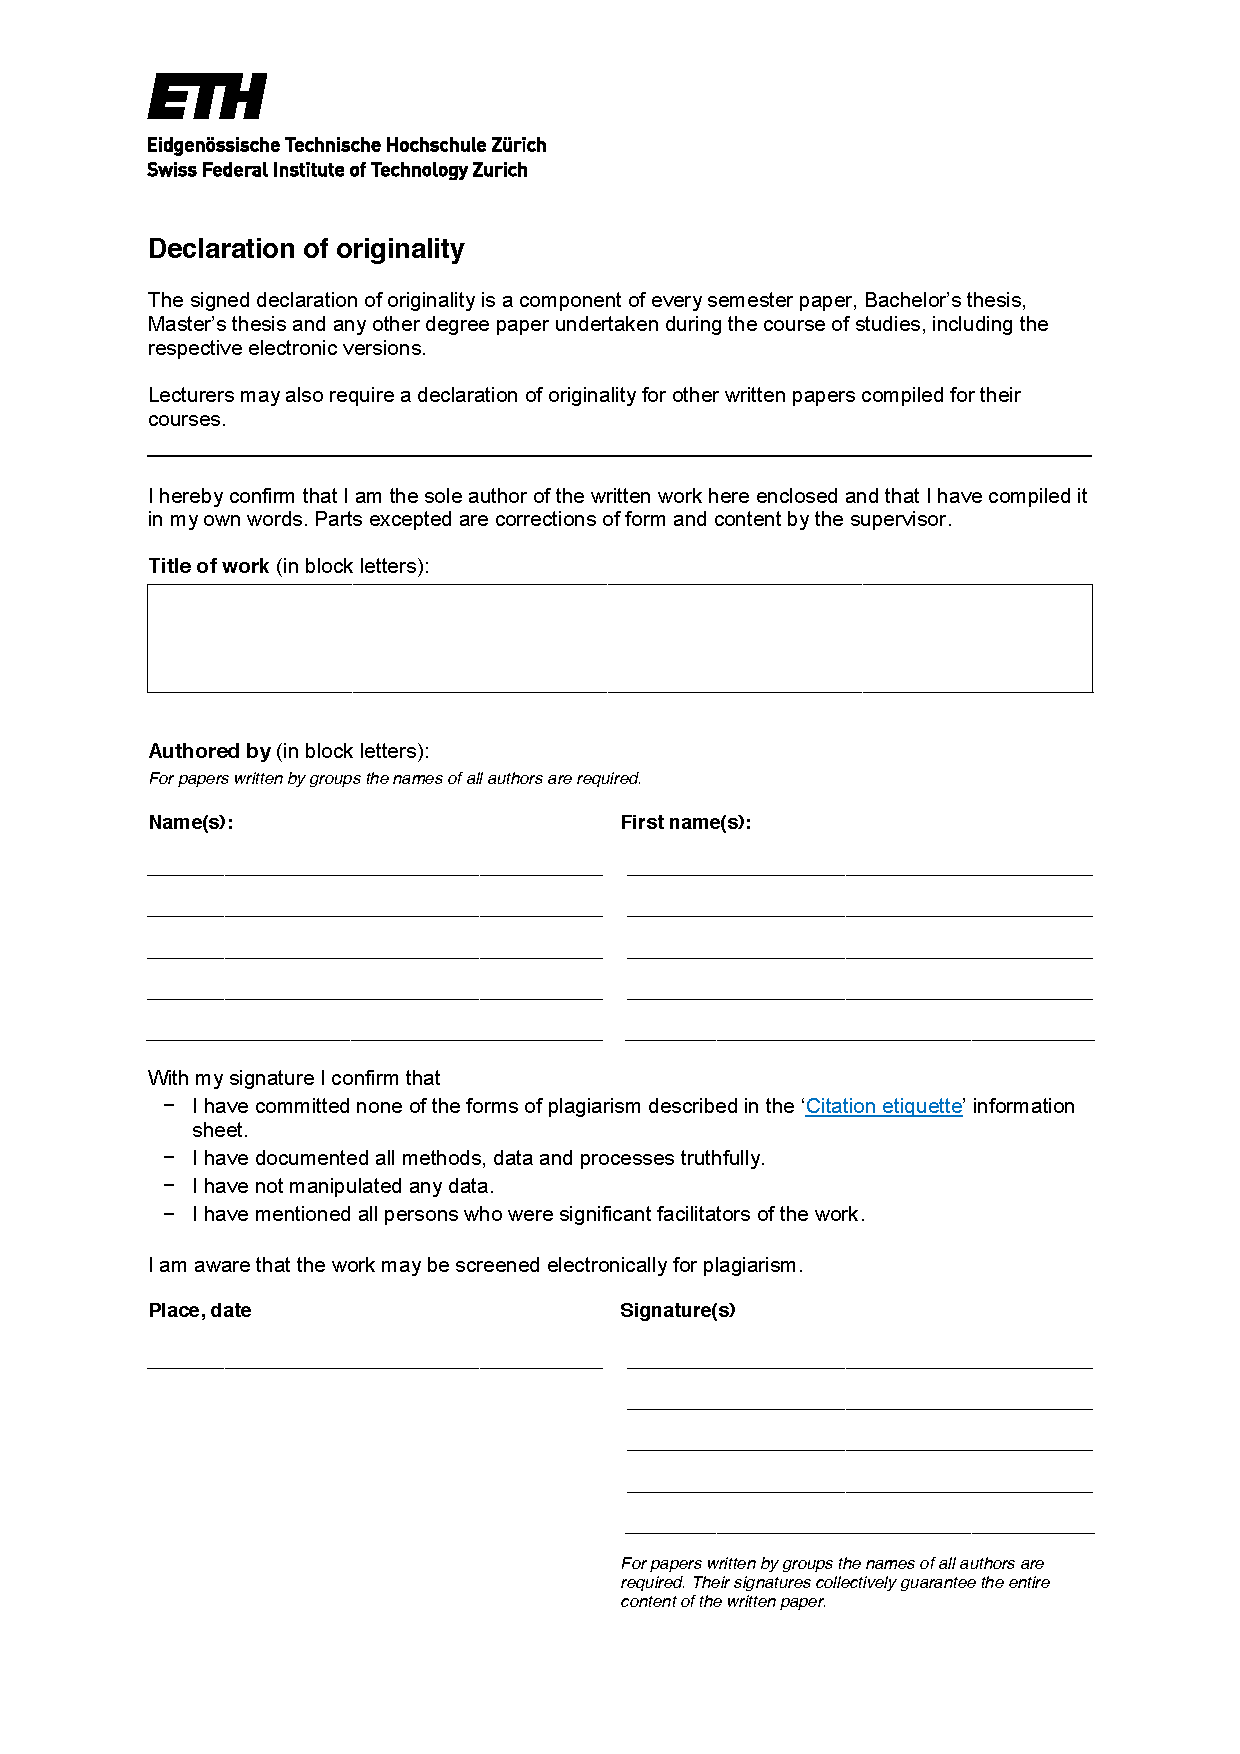
\includepdf[pages={-}]{utils/declaration-originality.pdf}

\end{document}
